\chapter{Method}
\label{ch:method}

\section*{Literature review}
I reviewed previous work, focusing on two areas. I explored already available
methods for creating animations from sketches by performing skeleton
classification and reviewed previous work dealing with the classification of
sketched objects.

\section*{Related work}
\textcite{eitz2012hdhso} collected a dataset of 20,000 sketches and divided them
into 250 categories of 80 images each. Humans recognized on average 73.1\% of 
these sketches correctly. This dataset is used in my work to train and validate
the classifier to choose which animation is the most appropriate to show.

\textcite{10.1145/3469877.3490565} proposes a pipeline to create rigged and
animated characters from a single image. Their solution aims for a holistic
approach, requiring no user intervention, to assist non-professional users in
creating animated characters. The proposed pipeline performs contour extraction
with salient object detection and extrudes a 3D mesh from geometry generated by
applying constrained Delaunay to the contours. Afterwards, a skeleton is
estimated using a mean curve method and an animation is transferred onto the
skeleton. In our work, we want to follow a similar philosophy of no user
interaction and hope to improve the believability of the animated results by not
only classifying the skeleton type but also the subject class of the input
sketch.

\section*{Training classification models}
We used a subset of the dataset provided by \textcite{eitz2012hdhso} and
\textcite{10.1145/2897824.2925954} to train our classification models.
Only the classes "cat" and "dog" were taken as training data for our models. 
To train and evaluate our models we used the scikit-learn library introduced by
\textcite{scikit-learn}.

\subsection*{kNN classifier}
We trained a kNN classifier with the pixel values of the input images. Before
using the values to train the model, we resized the images to a size of 64 times 
64 pixels, and flattened the array to get a feature vector with 12288 entries, 
ranging from 0 to 255 in value. To find the best-performing k, we performed a
grid search with cross-validation on 3 folds leading to k = 5 as the model with 
the highest accuracy at 61.8798\%.

\subsection*{SVM classifier}
We trained an SVM classifier with a total of 1544 labeled images of sketches of
cats and dogs. Before training the model we resized the images to a size of 64
times 64 pixels, and flattened the array to get a feature vector with 4480
entries. The images were imported as grayscale images. The SVM classifier
performed with an accuracy of 53.7578\%.


\subsection*{Neural network classifier}
We created and trained a Neural Network binary classifier using pytorch
\textcite{pytorch}. This is the network's setup:

\begin{lstlisting}
    class MyNN(nn.Module):
    def __init__(self):
        super().__init__()
        self.linear_relu_stack = nn.Sequential(
            nn.Linear(in_features=3*128*128,out_features=16*16),
            nn.ReLU(),
            nn.Linear(in_features=16*16,out_features=16*16),
            nn.ReLU(),
            nn.Linear(in_features=16*16,out_features=1)
        )
    def forward(self, x, **kwargs):
        x = x.view(x.size(0), -1)
        logits = self.linear_relu_stack(x)
        return logits
\end{lstlisting}

The network was trained on 80\% of a collection of in total 1544 labeled images,
depicting sketches of cats and dogs. The images where resized to a size of
128 times 128 pixels before being fed into the network. Training the network on
80\% of the dataset for 500 epochs with a loss rate of 0.0001, led to the
network performing with a 59.15\% accuracy on the unseen test data.

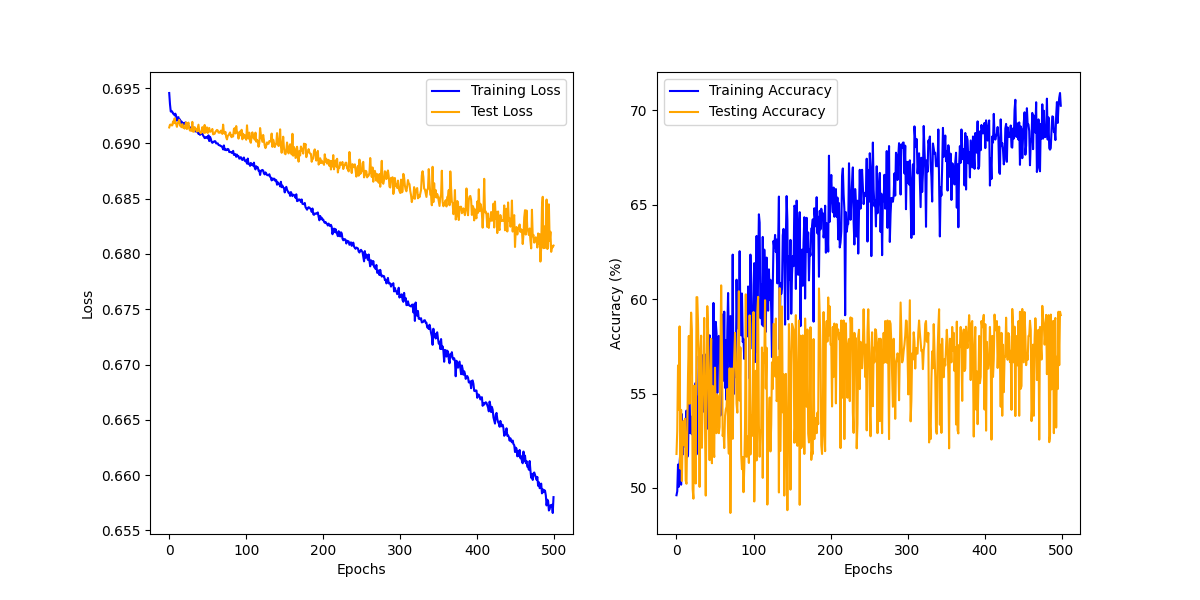
\includegraphics[width=\textwidth]{Figures/NN_classifier_charts.png}

\section*{Implementing the pipeline}
For this work, we reimplemented the pipeline proposed by
\textcite{korpitsch-2023-sao}, and adapted the code where needed.

\subsection*{Sketchdetection}
To repeat the steps introduced by \textcite{korpitsch-2023-sao} we collected the
dataset provided by \textcite{sarvadevabhatla2017sketchparse}. In
\textcite{smith2023method}, a Mask-R-CNN, as described by \textcite{he2018mask},
is used to detect the bounding boxes of figures drawn by children. 